\documentclass[11pt]{article}
\usepackage[T1]{fontenc}
\usepackage{amsmath,amssymb}
\usepackage{tikz}
\usetikzlibrary{arrows.meta}
\usepackage[paperwidth=16cm,paperheight=10.85cm,margin=0pt]{geometry}
\pagestyle{empty}
\definecolor{oo}{HTML}{D55E00}
\definecolor{og}{HTML}{999999}
\definecolor{ol}{HTML}{E1E9F1}
\definecolor{om}{HTML}{FBE3D2}
\begin{document}
\footnotesize
\noindent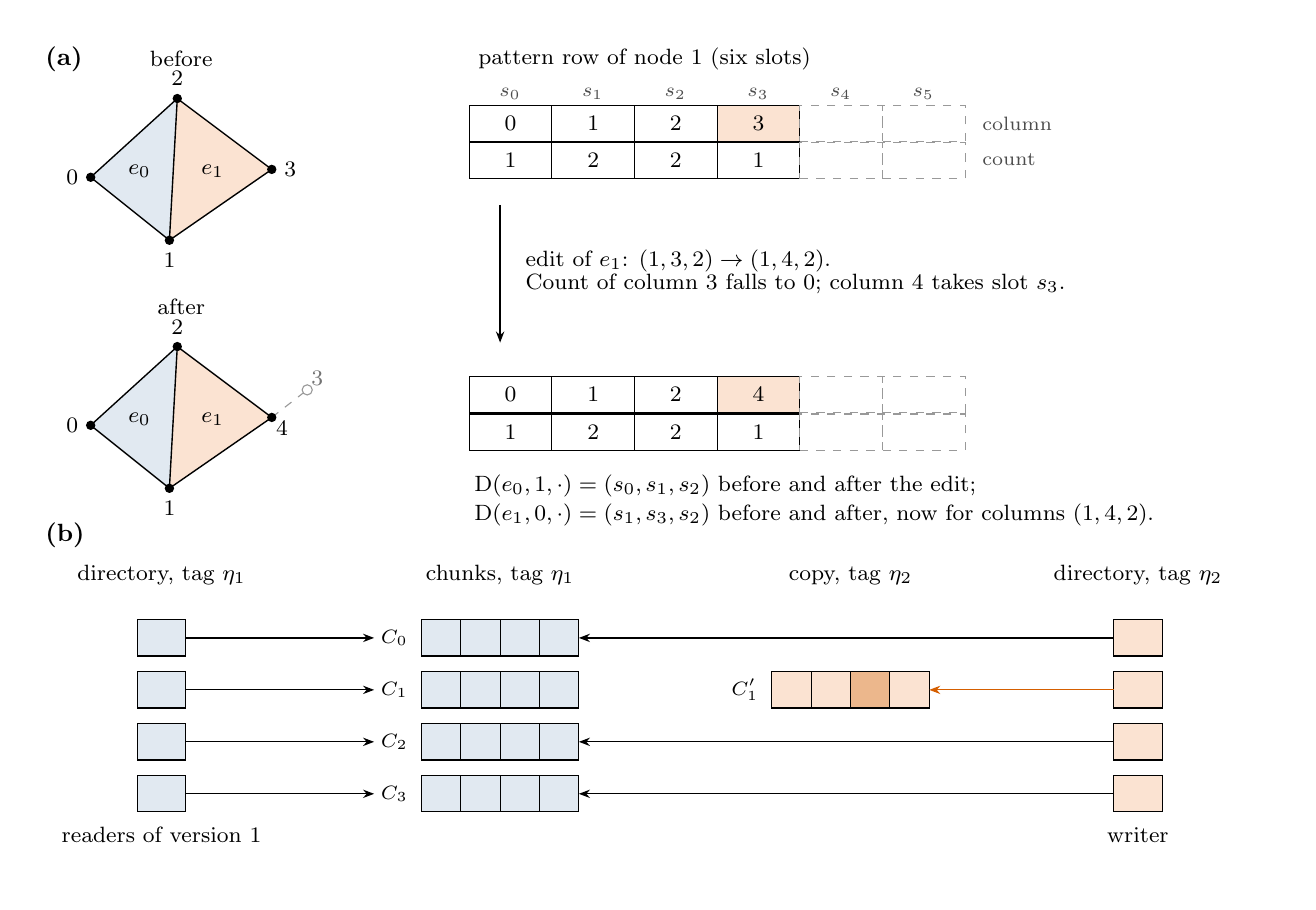
\begin{tikzpicture}[x=1cm,y=1cm,
  slot/.style={draw,minimum width=1.05cm,minimum height=0.46cm,inner sep=0pt,line width=0.4pt},
  cell/.style={draw,minimum width=0.62cm,minimum height=0.46cm,inner sep=0pt,line width=0.4pt},
  chk/.style={draw,minimum width=0.5cm,minimum height=0.46cm,inner sep=0pt,line width=0.4pt},
  node1/.style={circle,fill=black,inner sep=1.2pt},
  ptr/.style={-{Stealth[length=4pt,width=3pt]},line width=0.45pt},
  every node/.style={font=\footnotesize}]
\useasboundingbox (0,-0.65) rectangle (16,10.2);

%% ---------------- panel (a) ----------------
\node[anchor=west,font=\small\bfseries] at (0.1,9.8) {(a)};
\begin{scope}[shift={(0.8,8.3)}]
  \coordinate (n0) at (0.0,0.0); \coordinate (n1) at (1.0,-0.8); \coordinate (n2) at (1.1,1.0); \coordinate (n3) at (2.3,0.1);
  \fill[ol] (n0)--(n1)--(n2)--cycle;
  \fill[om] (n1)--(n3)--(n2)--cycle;
  \draw[line width=0.5pt] (n0)--(n1)--(n3)--(n2)--cycle; \draw[line width=0.5pt] (n1)--(n2);
  \foreach \n in {n0,n1,n2,n3}{\node[node1] at (\n) {};}
  \node[left=1pt] at (n0) {$0$}; \node[below=1pt] at (n1) {$1$}; \node[above=1pt] at (n2) {$2$}; \node[right=1pt] at (n3) {$3$};
  \node at (0.62,0.08) {$e_0$}; \node at (1.55,0.08) {$e_1$};
  \node at (1.15,1.5) {before};
\end{scope}
\begin{scope}[shift={(0.8,5.15)}]
  \coordinate (n0) at (0.0,0.0); \coordinate (n1) at (1.0,-0.8); \coordinate (n2) at (1.1,1.0); \coordinate (n4) at (2.3,0.1); \coordinate (n3) at (2.75,0.45);
  \fill[ol] (n0)--(n1)--(n2)--cycle;
  \fill[om] (n1)--(n4)--(n2)--cycle;
  \draw[line width=0.5pt] (n0)--(n1)--(n4)--(n2)--cycle; \draw[line width=0.5pt] (n1)--(n2);
  \draw[line width=0.4pt,dashed,og] (n4)--(n3);
  \foreach \n in {n0,n1,n2,n4}{\node[node1] at (\n) {};}
  \node[circle,draw=og,fill=white,inner sep=1.3pt,line width=0.4pt] at (n3) {};
  \node[left=1pt] at (n0) {$0$}; \node[below=1pt] at (n1) {$1$}; \node[above=1pt] at (n2) {$2$};
  \node[below right=-2pt] at (n4) {$4$}; \node[above right=-2pt,text=black!55] at (n3) {$3$};
  \node at (0.62,0.08) {$e_0$}; \node at (1.55,0.08) {$e_1$};
  \node at (1.15,1.5) {after};
\end{scope}

\def\sx{5.6}
\node[anchor=west] at (\sx,9.8) {pattern row of node $1$ (six slots)};
\foreach \i in {0,...,5}{\node[font=\scriptsize,text=black!70] at (\sx+1.05*\i+0.525,9.36) {$s_{\i}$};}
\def\yb{8.75}
\foreach \i/\c/\n/\f in {0/0/1/white,1/1/2/white,2/2/2/white,3/3/1/om}{
  \node[slot,fill=\f,anchor=south west] at (\sx+1.05*\i,\yb) {$\c$};
  \node[slot,anchor=north west] at (\sx+1.05*\i,\yb) {$\n$};}
\foreach \i in {4,5}{
  \node[slot,anchor=south west,dashed,draw=og] at (\sx+1.05*\i,\yb) {};
  \node[slot,anchor=north west,dashed,draw=og] at (\sx+1.05*\i,\yb) {};}
\node[anchor=west,font=\scriptsize,text=black!70] at (\sx+6.4,\yb+0.23) {column};
\node[anchor=west,font=\scriptsize,text=black!70] at (\sx+6.4,\yb-0.23) {count};
\def\ya{5.3}
\foreach \i/\c/\n/\f in {0/0/1/white,1/1/2/white,2/2/2/white,3/4/1/om}{
  \node[slot,fill=\f,anchor=south west] at (\sx+1.05*\i,\ya) {$\c$};
  \node[slot,anchor=north west] at (\sx+1.05*\i,\ya) {$\n$};}
\foreach \i in {4,5}{
  \node[slot,anchor=south west,dashed,draw=og] at (\sx+1.05*\i,\ya) {};
  \node[slot,anchor=north west,dashed,draw=og] at (\sx+1.05*\i,\ya) {};}
\draw[ptr,line width=0.7pt] (\sx+0.4,7.95) -- (\sx+0.4,6.2);
\node[anchor=west,align=left] at (\sx+0.6,7.1) {edit of $e_1$: $(1,3,2)\to(1,4,2)$.\\[-1pt]
 Count of column $3$ falls to $0$; column $4$ takes slot $s_3$.};
\node[anchor=north west,align=left] at (\sx-0.05,4.65) {$\mathrm{D}(e_0,1,\cdot)=(s_0,s_1,s_2)$ before and after the edit;\\[1pt]
 $\mathrm{D}(e_1,0,\cdot)=(s_1,s_3,s_2)$ before and after, now for columns $(1,4,2)$.};

%% ---------------- panel (b) ----------------
\node[anchor=west,font=\small\bfseries] at (0.1,3.75) {(b)};
\def\cx{6.0}\def\cy{2.45}\def\dy{0.66}
\node[anchor=south] at (1.7,3.0) {directory, tag $\eta_1$};
\node[anchor=south] at (\cx,3.0) {chunks, tag $\eta_1$};
\node[anchor=south] at (10.45,3.0) {copy, tag $\eta_2$};
\node[anchor=south] at (14.1,3.0) {directory, tag $\eta_2$};
\foreach \i in {0,1,2,3}{
  \pgfmathsetmacro{\y}{\cy-\dy*\i}
  \node[cell,fill=ol] at (1.7,\y) {};
  \node[cell,fill=om] at (14.1,\y) {};
  \foreach \j in {0,1,2,3}{\node[chk,fill=ol] at (\cx-0.75+0.5*\j,\y) {};}
  \node[anchor=east,font=\scriptsize] at (\cx-1.05,\y) {$C_{\i}$};
  \draw[ptr] (1.7+0.31,\y) -- (\cx-1.6,\y);
}
\foreach \i in {0,2,3}{
  \pgfmathsetmacro{\y}{\cy-\dy*\i}
  \draw[ptr] (14.1-0.31,\y) -- (\cx+1.0,\y);
}
\foreach \j in {0,1,2,3}{\node[chk,fill=om] at (10.45-0.75+0.5*\j,\cy-\dy) {};}
\node[chk,fill=oo!45] at (10.45-0.75+0.5*2,\cy-\dy) {};
\node[anchor=east,font=\scriptsize] at (10.45-1.05,\cy-\dy) {$C_1'$};
\draw[ptr,oo] (14.1-0.31,\cy-\dy) -- (10.45+1.0,\cy-\dy);
\node[anchor=north] at (1.7,\cy-3*\dy-0.3) {readers of version $1$};
\node[anchor=north] at (14.1,\cy-3*\dy-0.3) {writer};
\end{tikzpicture}
\end{document}
